% (c) 2012 Dimitrios Vrettos - d.vrettos@gmail.com
% (c) 2012 Claudio Carboncini - claudio.carboncini@gmail.com
% (c) 2014 Daniele Zambelli - daniele.zambelli@gmail.com

\section{Esercizi}

\subsection{Esercizi dei singoli paragrafi}

%\subsubsection*{5.1 - Insiemi ed elementi}
\subsubsection*{\numnameref{sec:insiemi_definizioni}}

\begin{esercizio}
 \label{ese:5.1}
 Barra con una crocetta i raggruppamenti che ritieni siano degli insiemi.
 \begin{multicols}{2}
 \begin{enumeratea}
\item I fiumi più lunghi d'Italia;
\item le persone con più di~30 anni;
\item i numeri~1, 20, 39, 43, 52;
\item i libri più pesanti nella tua cartella;
\item i punti di una retta;
\item gli animali con~2 zampe;
\item le vocali dell'alfabeto italiano;
\item i professori bravi;
\item i gatti con due code;
\item i calciatori che hanno fatto pochi gol.
\end{enumeratea}
\end{multicols}
\end{esercizio}

\begin{esercizio}
 \label{ese:5.2}
Per ciascuno dei seguenti casi inserisci il simbolo adatto fra ''$\in$'' e 
''$\notin$''. $A$ è l'insieme delle lettere
dell'alfabeto italiano. b \ldots $A$, i \ldots $A$, j \ldots $A$, e \ldots $A$, 
w \ldots $A$, z \ldots $A$
\end{esercizio}

\begin{esercizio}
\label{ese:5.3}
Le vocali delle parole che seguono formano insiemi uguali, tranne in un caso. 
Quale?
\begin{center}
 \boxA\quad sito\quad\boxB\quad micio\quad\boxC\quad zitto\quad\boxD\quad 
fiocco\quad\boxE\quad lecito\quad\boxF\quad dito.
\end{center}
\end{esercizio}

\begin{esercizio}
\label{ese:5.4}
Individua tra i seguenti insiemi quelli che sono uguali:
\begin{multicols}{2}
\begin{enumeratea}
 \item vocali della parola ``SASSO'';
 \item consonanti della parola ``SASSO'';
 \item vocali della parola ``PIETRA'';
 \item vocali della parola ``PASSO''.
\end{enumeratea}
\end{multicols}
\end{esercizio}

\begin{esercizio}
\label{ese:5.5}
Quali delle seguenti frasi rappresentano criteri oggettivi per individuare un 
insieme? Spiega perché.
\TabPositions{8.5cm}
\begin{enumeratea}
\item Le città che distano meno di~100 Km da Lecce; \tab\boxV\quad\boxF
\item i laghi d'Italia;  \tab\boxV\quad\boxF
\item le città vicine a Roma; \tab\boxV\quad\boxF
\item i calciatori della Juventus;  \tab\boxV\quad\boxF
\item i libri di Mauro;  \tab\boxV\quad\boxF
\item i professori bassi della tua scuola;  \tab\boxV\quad\boxF
\item i tuoi compagni di scuola il cui nome inizia per M; \tab\boxV\quad\boxF
\item i tuoi compagni di classe che sono gentili; \tab\boxV\quad\boxF
\item gli zaini neri della tua classe.  \tab\boxV\quad\boxF
\end{enumeratea}
\end{esercizio}

\begin{esercizio}
\label{ese:5.6}
Scrivi al posto dei puntini il simbolo mancante tra ''$\in$'' e ''$\notin$''.

\begin{enumeratea}
\item La Polo \ldots\ldots all'insieme delle automobili Fiat;
\item il cane \ldots\ldots all'insieme degli animali domestici;
\item la Puglia \ldots\ldots all'insieme delle regioni italiane;
\item Firenze \ldots\ldots all'insieme delle città francesi;
\item il numero~10 \ldots\ldots all'insieme dei numeri naturali;
\item il numero~3 \ldots\ldots all'insieme dei numeri pari.
\end{enumeratea}
\end{esercizio}

\begin{esercizio}
\label{ese:5.7}
Quali delle seguenti proprietà sono caratteristiche per un insieme?
\TabPositions{8.5cm}
\begin{enumeratea}
\item Essere città italiana il cui nome inizia per W; \tab\boxV\quad\boxF
\item essere un bravo cantante; \tab\boxV\quad\boxF
\item essere un monte delle Alpi;  \tab\boxV\quad\boxF
\item essere un ragazzo felice; \tab\boxV\quad\boxF
\item essere un numero naturale grande;\tab\boxV\quad\boxF
\item essere un ragazzo nato nel~1985; \tab\boxV\quad\boxF
\item essere gli alunni della classe~$1^{a}C$; \tab\boxV\quad\boxF
\item essere le lettere dell'alfabeto inglese; \tab\boxV\quad\boxF
\item essere le rette del piano; \tab\boxV\quad\boxF
\item essere i libri interessanti della biblioteca; \tab\boxV\quad\boxF
\item essere gli italiani viventi nati nel~1850; \tab\boxV\quad\boxF
\item essere gli italiani colti. \tab\boxV\quad\boxF
\end{enumeratea}
\end{esercizio}

\begin{esercizio}
\label{ese:5.8}
Scrivi al posto dei puntini il simbolo mancante tra ''$=$'' e ''${\neq}$''.
\begin{enumeratea}
\item L'insieme delle lettere della parola ``CANE'' e della parola ``PANE'' sono 
\ldots\ldots;
\item l'insieme delle vocali della parola ``INSIEME'' e della parola ``MIELE'' 
sono \ldots\ldots;
\item l'insieme delle consonanti della parola ``LETTO'' e della parola ``TETTO'' 
sono \ldots\ldots;
\item l'insieme delle lettere della parola ``CONTRO'' e della parola ``TRONCO'' 
sono \ldots\ldots;
\item l'insieme delle vocali della parola ``LIBRO'' e della parola ``MINISTRO'' 
sono \ldots\ldots;
\item l'insieme delle vocali della parola ``DIARIO'' e della parola ``RAMO'' 
sono \ldots\ldots;
\item l'insieme delle lettere della parola ``MOUSE'' e della parola ``MUSEO'' 
sono \ldots\ldots;
\item l'insieme delle consonanti della parola ``SEDIA'' e della parola 
``ADESSO'' sono \ldots\ldots;
\item l'insieme dei numeri pari minori di~5 e l'insieme vuoto sono \ldots\ldots;
\item l'insieme dei numeri pari e l'insieme dei multipli di~2 sono \ldots\ldots
\end{enumeratea}
\end{esercizio}

\begin{esercizio}
\label{ese:5.9}
Le stelle dell'universo formano un insieme, le stelle visibili a occhio nudo 
formano un insieme? Spiega il tuo punto di vista.
\end{esercizio}

%\subsubsection*{5.2 - Insieme vuoto, insieme universo, cardinalità}
%\subsubsection*{\numnameref{sec:05_cardinalita}}

\begin{esercizio}
\label{ese:5.10}
Indica se gli insiemi~$G =\text{\{gatti con~6 zampe\}}$ e~$P = \text{\{polli 
con~2 zampe\}}$ sono o non sono vuoti.
\end{esercizio}

\begin{esercizio}
\label{ese:5.11}
Barra con una croce gli insiemi vuoti.
\begin{enumeratea}
 \item L'insieme dei numeri positivi minori di~0;
 \item l'insieme dei numeri negativi minori di~100;
 \item l'insieme dei numeri pari minori di~100;
 \item l'insieme delle capitali europee della regione Lombardia;
 \item l'insieme dei triangoli con quattro angoli;
 \item l'insieme delle capitali italiane del Lazio
 \item l'insieme dei punti di intersezione di due rette parallele.
 \end{enumeratea}
\end{esercizio}

\begin{esercizio}
\label{ese:5.12}
Quali delle seguenti scritture sono corrette per indicare
l'insieme vuoto?
\begin{center}
 \boxA\quad~$\emptyset $ \quad\boxB\quad~0 \quad\boxC\quad~$\{\emptyset \}$ 
\quad\boxD\quad~$\{0\}$ \quad\boxE\quad \{ \}.
\end{center}
\end{esercizio}

\begin{esercizio}
\label{ese:5.13}
Quali dei seguenti insiemi sono vuoti? Per gli insiemi non vuoti indica la 
cardinalità.
\begin{enumeratea}
\item L'insieme degli uccelli con~6 ali;
\item l'insieme delle lettere della parola ``VOLPE'';
\item l'insieme dei cani con~5 zampe;
\item l'insieme delle vocali della parola ``COCCODRILLO'';
\item l'insieme delle vocali dell'alfabeto italiano;
\item l'insieme degli abitanti della luna;
\item l'insieme dei numeri sulla tastiera del telefonino.
\end{enumeratea}
\end{esercizio}

\begin{esercizio}
\label{ese:5.14}
Scrivi per ciascun insieme un possibile insieme universo.
\begin{enumeratea}
\item l'insieme dei rettangoli;
\item l'insieme dei multipli di~3;
\item l'insieme delle lettere della parola ``MATEMATICA'';
\item l'insieme dei libri di matematica;
\item l'insieme dei ragazzi che hanno avuto un'insufficienza in matematica.
\end{enumeratea}
\end{esercizio}

\begin{esercizio}
\label{ese:5.15}
Dato l'insieme~$A = {\{0, 3, 5\}}$ determina se le seguenti affermazioni sono 
vere o false.
\TabPositions{2.5cm}
\begin{enumeratea}
\item $0\in A$ \tab\boxV\quad\boxF
\item $5\in A$ \tab\boxV\quad\boxF
\item $\emptyset \in A$ \tab\boxV\quad\boxF
\item $\emptyset\in A$ \tab\boxV\quad\boxF
\item $A\in A$ \tab\boxV\quad\boxF
\item $3,5\in A$ \tab\boxV\quad\boxF
\end{enumeratea}
\end{esercizio}

% --------------------- Rappresentazione ---------------------

%\subsubsection*{6.1 - Rappresentazione tabulare}
\subsubsection*{\numnameref{sec:insiemi_rappresentazione}}

\begin{esercizio}
\label{ese:6.1}
Dai una rappresentazione tabulare dell'insieme~$A$ dei numeri naturali minori 
di~6.
\end{esercizio}

\begin{esercizio}
\label{ese:6.2}
Dai una rappresentazione tabulare dei seguenti insiemi
\begin{enumeratea}
 \item delle vocali della parola ``ESERCIZI'';
 \item delle lettere della parola ``RIFLETTERE'';
 \item dei numeri naturali compresi tra~6 e~12, estremi esclusi;
 \item dei numeri dispari compresi tra~10 e~20;
 \item delle lettere dell'alfabeto italiano;
 \item dei numeri naturali minori di~10;
 \item dei multipli di~7;
 \item delle preposizioni con più di due lettere.
\end{enumeratea}
\end{esercizio}

\begin{esercizio}
 \label{ese:6.3}
Indica in rappresentazione tabulare i seguenti insiemi.
\TabPositions{7.5cm}
\begin{enumeratea}
 \item $A=\{x\in\insN/x<10\}$\tab\dotfill
 \item $B=\{x\in\insN/2\le x<5\}$\tab\dotfill
 \item $C=\{x\in\insN/5\le x\le~10\}$\tab\dotfill
 \item $D=\{x\in\insN/2x\le~10\}$ \tab\dotfill
 \item $E=\{e\in\insN/5\le e<10\}$\tab\dotfill
 \item $F=\{f\in\insN/f\text{ è multiplo di~3 e } f<15\}$\tab\dotfill
 \item $G=\{g\in\insN/g\text{ è una cifra del numero }121231\}$\tab\dotfill
 \item $H=\{h\in\insN/h=3n+1,\text{ con }n\in\insN\}$\tab\dotfill
\end{enumeratea}
\end{esercizio}

\begin{esercizio}
\label{ese:6.4}
Elenca per tabulazione gli elementi di~$A=\{x|x\in\insN, x\text{ è pari, 
}x\leq10, x\neq0\}.$
\end{esercizio}

\begin{esercizio}
\label{ese:6.5}
Elenca per tabulazione gli elementi di~$L=\{l\text{ è una lettera della parola 
MATEMATICA}\}$
\end{esercizio}

%\subsubsection*{6.2 - Rappresentazione caratteristica}
%\subsubsection*{\numnameref{sec:06_caratteristica}}

\begin{esercizio}
\label{ese:6.6}
Descrivi mediante la proprietà caratteristica
l'insieme~$D= \{\text{S, T, U, D, I, A, R, E}\}$
\[D=\{x/ x\text{ è }\ldots\}\]
\end{esercizio}


\begin{esercizio}
\label{ese:6.7}
Descrivi mediante la proprietà caratteristica l'insieme
\[X=\{1, 2, 3, 4, 5, 6, 7, 8, 9, 10, 11, 12, 13, 14, 15\}.\]
\[X=\{x\in\insN/x\ldots\}\]
\end{esercizio}

\begin{esercizio}
\label{ese:6.8}
Descrivi mediante la proprietà caratteristica l'insieme dei numeri primi minori 
di~1000.
\end{esercizio}

\begin{esercizio}
\label{ese:6.9}
Elenca gli elementi dell'insieme~$I=\{n\in\insN/n\text{ è divisore di }12\}$
\end{esercizio}

\begin{esercizio}
\label{ese:6.10}
Elenca gli elementi dell'insieme~$I=\{n\in\insN/n\text{ è multiplo di~3 minore 
di }20\}$
\end{esercizio}

% \newpage

\begin{esercizio}
\label{ese:6.11}
Dato l'insieme~$A=\{2, 4, 8, 16, 32, 64\}$ quale delle seguenti proprietà 
caratterizzano i suoi elementi?
\begin{enumeratea}
\item $A=\{n\in\insN/n \text{ è numero pari minore di }65\}$
\item $A=\{n\in\insN/n\text{ è una potenza di }2\}$
\item $A=\{n\in\insN/n\text{ è una potenza di~2 minore di }65\}$
\item $A=\{n\in\insN/n=2^{m},\text{ con }m=1,2,3,4,5,6\}$
\end{enumeratea}
\end{esercizio}

\begin{esercizio}
\label{ese:6.12}
Indica con una proprietà caratteristica l'insieme~$B=\{5, 10, 15, 20, 25, 30, 
35, 40, 45, 50\}$
\end{esercizio}

\begin{esercizio}
\label{ese:6.13}
Indica con una proprietà caratteristica
l'insieme~$B=\{4, 9, 16, 25, 36, 49, 64, 81\}$
\end{esercizio}

\begin{esercizio}
\label{ese:6.14}
Quale delle seguenti frasi indica la proprietà caratteristica
di~$A=\{0, 4, 8, 12, 16, 20, \ldots\}$
\begin{center}
\boxA\quad I multipli di~2; \quad\boxB\quad i numeri pari; \quad\boxC\quad i 
multipli di~4; \quad\boxD\quad i divisori di~20
\end{center}
\end{esercizio}

\begin{esercizio}
\label{ese:6.15}
Rappresenta in forma caratteristica i seguenti insiemi.
\begin{enumeratea}
\item $A=\{5, 6, 7, 8, 9, 10\}$
\item $B=\{0, 1, 2, 3, 4, 5, \dots, 98, 99, 100\}$
\item$ C=\{0, 3, 6, 9, 12, 15, 18, 21, 24, 27, 30\}$
\end{enumeratea}
\end{esercizio}

\begin{esercizio}
\label{ese:6.16}
Quale delle seguenti è una rappresentazione per caratteristica
dell'insieme
\[D = \{0, 3, 6, 9, 12, 15, 18\}.\]
\begin{multicols}{2}
\begin{enumeratea}
\item $D=\{x\in\insN/x\leqslant~18\}$
\item $D=\{x\in\insN/x\text{ è multiplo di~3 e }x<20\}$%
\item $D=\{x\in\insN/x=3x\}$
\item $D=\{x\in\insN/x=3\}$
\end{enumeratea}
\end{multicols}
\end{esercizio}

\begin{esercizio}
\label{ese:6.17}
Rappresenta i seguenti insiemi con la proprietà caratteristica.
\begin{enumeratea}
 \item $A=\{\text{gennaio, maggio, giugno, luglio, agosto}\}$
 \item $B=\{\text{Gorizia, Pordenone, Trieste, Udine}\}$
 \item $C=\{\text{sabato, domenica}\}$
 \item $D=\{10, 20, 30, 40, 50\}$
 \item $E=\{\text{Puglia, Piemonte}\}$
 \end{enumeratea}
\end{esercizio}

\begin{esercizio}
Individua una proprietà caratteristica dei seguenti insiemi numerici.
\label{ese:6.18}
\begin{multicols}{2}
\begin{enumeratea}
\spazielenx
 \item $A=\{4,9,16,25,\ldots\}$
 \item 
$B=\bigg\{\dfrac{1}{4},\dfrac{1}{9},\dfrac{1}{16},\dfrac{1}{25},\ldots\bigg\}$
 \item 
$C=\bigg\{2,\dfrac{3}{2},\dfrac{4}{3},\dfrac{5}{4},\dfrac{6}{5},\ldots\bigg\}$
 \item 
$D=\bigg\{\dfrac{1}{5},\dfrac{1}{10},\dfrac{1}{15},\dfrac{1}{20},\ldots\bigg\}$
 \item 
$E=\bigg\{\dfrac{1}{4},\dfrac{2}{9},\dfrac{3}{16},\dfrac{4}{25},\dfrac{5}{36},
\ldots\bigg\}$
 \item $F=\{+1, -2, +4, -8, +16, -32, +64, \ldots\}$
 \end{enumeratea}
\end{multicols}
\end{esercizio}

\begin{esercizio}
\label{ese:6.19}
Elenca gli elementi dei seguenti insiemi.
\begin{multicols}{2}
\begin{enumeratea}
\item $A=\{x\in\insZ/-3\le x<2\}$
\item $B=\{x\in\insN/-4\le x\le~1\text{ o }5<x\le~7\}$
\end{enumeratea}
\end{multicols}
\end{esercizio}

\begin{esercizio}
\label{ese:6.20}
Rappresenta in forma caratteristica i seguenti insiemi.
\begin{enumeratea}
\item $A=\{0, 2, 4, 6, 8, 10\}$
\item $B=\{1, 4, 9, 16, 25, 36,49, \ldots\}$
\item $C=\{3, 4, 5, 6, 7\}$
\item $D=\{-5, -4, -3, -2, -1, 0, +1, +2, +3, +4, +5\}$
\item $E=\{0, 10, 20, 30, 40, 50, 60, 70, 80, 90, 100\}$
\item $F=\{1, 4, 9, 16, 25, 36, 49, 64, 81, 100\}$
\end{enumeratea}
\end{esercizio}

%\subsubsection*{6.3 - Rappresentazione grafica (Diagramma di Venn)}
%\subsubsection*{\numnameref{sec:06_venn}}

\begin{esercizio}
\label{ese:6.21}
Rappresenta con un diagramma di Eulero-Venn l'insieme:
\begin{enumeratea}
\item dei multipli di~3 compresi tra~10 e~30, estremi inclusi;
\item delle note musicali;
\item dei numeri primi minori di~20;
\item delle consonanti della parola ``MATEMATICA'';
\item delle province della Toscana.
\end{enumeratea}
\end{esercizio}

\begin{esercizio}
\label{ese:6.22}
In base agli insiemi~$A$ e~$B$ rappresentati dai diagrammi di Venn, stabilisci 
quali affermazioni sono vere.
\begin{multicols}{2}
\TabPositions{2.5cm}
\begin{enumeratea}
\item $5\notin B$\tab\boxV\quad\boxF
\item $A=\emptyset $\tab\boxV\quad\boxF
\item $3+2\in A$\tab\boxV\quad\boxF
\item $B\neq \emptyset $\tab\boxV\quad\boxF
\item $6\in B$\tab\boxV\quad\boxF
\item $9\notin A$\tab\boxV\quad\boxF
\end{enumeratea}
\columnbreak
% (c) 2012 Dimitrios Vrettos - d.vrettos@gmail.com
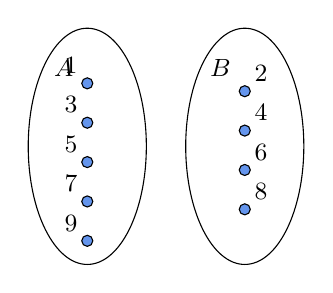
\begin{tikzpicture}[x=.5cm,y=1cm,font=\small]
    \draw (0,0)circle (1.5) (0,1) node[ left=1.5] {$A$};
    \begin{scope}[fill=CornflowerBlue, draw=black]
\filldraw (0,.8) circle (2pt) node[above left] {1};
\filldraw (0,.3) circle (2pt) node[above left] {3};
\filldraw (0,-.2) circle (2pt) node[above left] {5};
\filldraw (0,-.7) circle (2pt) node[above left] {7};
\filldraw (0,-1.2) circle (2pt) node[above left] {9};
\begin{scope}[xshift=2cm]
    \draw (0,0)circle (1.5) (0,1) node[ left=1.5] {$B$};
\filldraw (0,.7) circle (2pt) node[above right] {2};
\filldraw (0,.2) circle (2pt) node[above right] {4};
\filldraw (0,-.3) circle (2pt) node[above right] {6};
\filldraw (0,-.8) circle (2pt) node[above right] {8};
\end{scope}
\end{scope}
\end{tikzpicture}

\end{multicols}
\end{esercizio}

% --------------------- Operazioni ---------------------

%\subsubsection*{7.1 - Sottoinsieme}
\subsubsection*{\numnameref{sec:insiemi_operazioni}}

\begin{esercizio}
\label{ese:7.1}
 Siano~$T=\{t / t\text{ un triangolo}\}$, $R=\{r / r\text{ un rettangolo}\}$,
$E=\{e / e\text{ un triangolo equilatero}\}$ Quale affermazione è vera?
\begin{multicols}{4}
\begin{enumeratea}
\item $R\subset T$
\item $E\subset T$
\item $E\subset R$
\item $T\subset E$
\end{enumeratea}
\end{multicols}
\end{esercizio}

%\subsubsection*{7.2 - Insieme delle parti}
%\subsubsection*{\numnameref{sec:07_parti}}

\begin{esercizio}
\label{ese:7.2}
Se~$A=\{x\in\insN/1\le x<3\}$, allora~$\wp (A)$ ha:
\begin{center}
\boxA\quad~2 elementi,\quad\boxB\quad~3 elementi,\quad\boxC\quad~4 
elementi,\quad\boxD\quad~8 elementi
\end{center}
\end{esercizio}

\begin{esercizio}
 \label{ese:7.3}
Considera l'insieme~$B=\{x\in\insN/1<x<5\}$
e~$\wp (B)$ Quali delle seguenti affermazioni sono vere o false?
\begin{multicols}{2}
\TabPositions{4cm}
\begin{enumeratea}
 \item $\{1\}\in\wp (B)$ \tab\boxV\quad\boxF
 \item $\emptyset\subset\wp (B)$ \tab\boxV\quad\boxF
 \item $\{2,5\}\in\wp (B)$ \tab\boxV\quad\boxF
 \item $\{\emptyset\}\in\wp (B)$ \tab\boxV\quad\boxF
 \item $0\in\emptyset $ \tab\boxV\quad\boxF
 \item $\emptyset\subseteq B$ \tab\boxV\quad\boxF
 \item $\{1,2,3\}\in\wp (B)$ \tab\boxV\quad\boxF
 \item $\{1,2,3\}\notin\wp (B)$ \tab\boxV\quad\boxF
\end{enumeratea}
\end{multicols}
\end{esercizio}

\begin{esercizio}
 \label{ese:7.4}
 Scrivi l'insieme che ha come insieme delle parti
$\{\emptyset,\{8,10\},\{8\},\{10\}\}$
\end{esercizio}

\begin{esercizio}
 \label{ese:7.5}
Dato~$H=\{h/\text{h è una lettera della parola ``MAMMA''}\}$ scrivi
tutti gli elementi di~$\wp (H)$
\end{esercizio}

\begin{esercizio}
 \label{ese:7.6}
 Dato~$A=\{x\in\insN/ n<5\text{ e }n\text{ divisore di~12}\}$ scrivi tutti gli 
elementi di
$\wp (A)$
\end{esercizio}

%\subsubsection*{7.3 - Insieme unione}
%\subsubsection*{\numnameref{sec:07_unione}}

\begin{esercizio}
 \label{ese:7.7}
Dati~$A=\{1,2,4,5\}$ e~$B=\{1,3,4,5,8\}$ determina la loro unione dopo
aver rappresentato gli insiemi mediante diagrammi di Eulero-Venn.
 \end{esercizio}

\begin{esercizio}
 \label{ese:7.8}
 Dati gli insiemi~$L=\{1,2,5,6,7,8\}$, $M=\{4,5,6,7,10\}$ e~$N=\{2,3,5,7,9,10\}$
determina l'insieme unione completando prima la rappresentazione
grafica poi quella tabulare.
\begin{center}
 % (c) 2012 Dimitrios Vrettos - d.vrettos@gmail.com
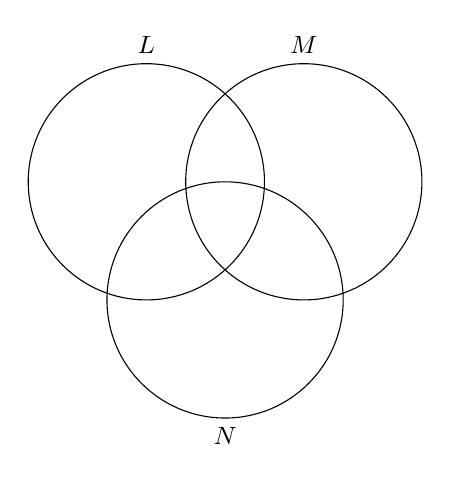
\begin{tikzpicture}[font=\small]
\draw (0,0)circle (1.5) (0,1.5) node[above] {$L$};
\draw(2,0) circle (1.5) (2,1.5) node [above]  {$M$};
\draw(1,-1.5)circle (1.5) (1,-3) node[below]{$N$};
\end{tikzpicture}

\end{center}
\end{esercizio}

% \begin{esercizio}
%  \label{ese:7.9}
% Dati gli insiemi~$C$ delle lettere della parola ``GIARDINO'' e~$D$ delle lettere 
% della
% parola ``ORA'', determina la loro unione aiutandoti con la rappresentazione 
% grafica.
%  \end{esercizio}
% 
% %\subsubsection*{7.4 - Insieme intersezione}
% %\subsubsection*{\numnameref{sec:07_intersezione}}
% 
%  \begin{esercizio}
%  \label{ese:7.10}
% Dati~$A=\{1,2,4,5\}$ e~$B=\{1,3,4,5,8\}$ determina la loro
% intersezione dopo aver rappresentato gli insiemi mediante diagrammi di
% Eulero-Venn.
% \end{esercizio}
% 
% \begin{esercizio}
%  \label{ese:7.11}
% Dati gli insiemi~$C$ delle lettere della parola ``LIBRO'' e~$D$ delle lettere 
% della
% parola ``PASTA'' determina la loro intersezione aiutandoti con la 
% rappresentazione grafica.
% \end{esercizio}

\begin{esercizio}
 \label{ese:7.12}
Considerando i~3 insiemi~$S=\{\text{a, b, c, e, f, s, t}\}$, $T=\{\text{a, c, g, 
h, l, s}\}$ e~$U=\{\text{b, c, d, g, s, t}\}$,
determina l'insieme intersezione dando sia la rappresentazione grafica sia 
quella tabulare.
 \end{esercizio}

\begin{esercizio}
 \label{ese:7.13}
 Determina l'intersezione tra i seguenti insiemi:
\begin{enumeratea}
 \item $A=\{-3, -2, -1, 0, +1, +2, +3\}$, $B=\{-2,-1, 0, +1, +2, +3, +4\}$ 
$A\cap B=\ldots$
 \item $A=\{x\in\insN/2\le x\le~5\}$, $B=\{x\in\insN/3<x<7\}$ $B\cap A=\ldots$
 \item $A=\{x\in\insZ/-5\le x\le+5\}$, $B=\{x\in\insZ/-15\le x<3\}$ $A\cap 
B=\ldots$
 \item $A=\{x\in\insN/x>100\}$, $B=\{x\in\insN/10<x<20\}$ $B\cap A=\ldots$
 \item $A=\{l\text{ lettera di ``SATURNO''}\}$, $B=\{l\text{ lettera di 
``NETTUNO''}\}$ $A\cap B=\ldots$
\end{enumeratea}
\end{esercizio}

%\subsubsection*{7.5 - Insieme differenza}
%\subsubsection*{\numnameref{sec:07_differenza}}

\begin{esercizio}
\label{ese:7.14}
Dati gli insiemi~$E=\{x / x$ è una lettera della parola ``cartellone''\} e
$F=\{x / x$ è una lettera della parola ``martello''\}, determina
$E-F$ e~$F-E$
\end{esercizio}

%\subsubsection*{7.5 - Insieme complementare}
%\subsubsection*{\numnameref{sec:07_complementare}}

\begin{esercizio}
\label{ese:7.15}
Verifica, utilizzando la rappresentazione grafica, che
% \begin{multicols}{2}
 \begin{enumeratea}
 \item $\overline{A}_{U}\cup A=U$
 \item $(A-B)\cup (B-A)\cup (\overline{A\cup B})=\overline{{A\cap B}}$
 \end{enumeratea}
% \end{multicols}
\end{esercizio}

\begin{esercizio}
 \label{ese:7.16}
Dati~$E$ ed~$F$ sottoinsiemi di un insieme~$U$, l'insieme
definito da~$\overline{E\cap F}$ è uguale a:
\begin{center}
\boxA\quad~$E\cup F$\quad\boxB\quad~$\overline{E\cup F}$\quad\boxC\quad~$E\cap 
F$\quad\boxD\quad~$\overline{E}\cup\overline{F}$
\end{center}
\end{esercizio}

\begin{esercizio}
 \label{ese:7.17}
Dati~$G$ ed~$H$ sottoinsiemi di un insieme~$U$, l'insieme
definito da~$\overline{G\cup H}$ è uguale a:
\begin{center}
\boxA\quad~$\overline{{G\cap 
H}}$\quad\boxB\quad~$\overline{G}\cap\overline{H}$\quad\boxC\quad~$\overline{{
G\cap \overline{H}}}$\quad\boxD\quad nessuno dei precedenti
\end{center}
\end{esercizio}

%\subsubsection*{7.6 - Leggi di De Morgan}
%\subsubsection*{\numnameref{sec:07_demorgan}}

\begin{esercizio}
 \label{ese:7.18}
 Dimostra la seconda legge di De Morgan, annerendo gli spazi opportuni.
 \begin{center}
 %\usetikzlibrary{decorations.markings}
%\usetikzlibrary{matrix,fit}
%\usetikzlibrary{positioning}
%\usetikzlibrary{shapes.geometric}
%\usetikzlibrary{decorations.pathreplacing}
%\usetikzlibrary{decorations.text}
%\usetikzlibrary{mindmap}
%\usetikzlibrary{plotmarks}
%\usetikzlibrary{backgrounds}
%\usetikzlibrary{patterns}

% (c) 2012 Dimitrios Vrettos - d.vrettos@gmail.com

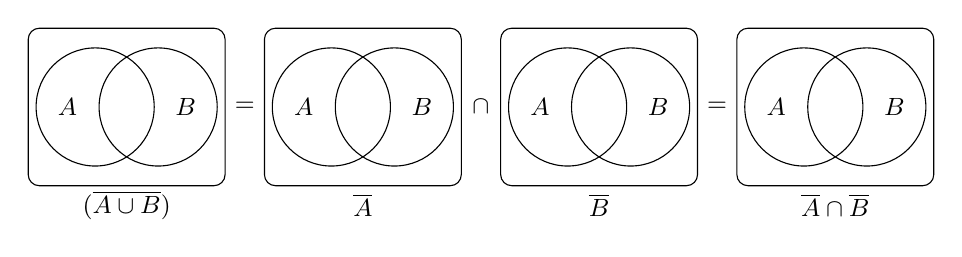
\begin{tikzpicture}[x=5mm,y=5mm,font=\small, outline/.style={draw=circle edge}]
\definecolor{circle area}{gray}{0.9}
\definecolor{circle edge}{rgb}{0,0,0}

\def\firstcircle{(1.7,2) circle (1.5)}
\def\secondcircle{(3.3,2) circle (1.5)}

\begin{scope}[rounded corners]
\foreach \i in {0,6,12,18}
\draw[fill=white] (\i,0) rectangle (\i+5,4);
\end{scope}

\begin{scope}]
\begin{scope}
\clip \firstcircle;
\fill[white] \secondcircle;
\end{scope}
\draw[outline] \firstcircle;
\draw[outline] \secondcircle;
\end{scope}

\begin{scope}[xshift=30mm]
\begin{scope}
\clip \firstcircle;
\fill[white] \firstcircle;
\end{scope}
 \draw[outline]  \firstcircle;
\draw[outline] \secondcircle;
\end{scope}

\begin{scope}[xshift=60mm]
\begin{scope}
\clip \secondcircle;
\fill[white] \secondcircle;
\end{scope}
 \draw[outline]  \firstcircle;
\draw[outline] \secondcircle;
\end{scope}

\begin{scope}[xshift=90mm]
\begin{scope}
\clip \firstcircle;
\fill[white] \secondcircle;
\end{scope}
\draw[outline] \firstcircle;
 \draw[outline] \secondcircle;
\end{scope}

\foreach \x/\xtext in {5.5/$=$,11.5/$\cap$,17.5/$=$}
	\node  at (\x,2) {\xtext};

\foreach \y in {1,7,13,19}
\node  at (\y,2) {$A$};

\foreach \z in {4,10,16,22}
\node  at (\z,2) {$B$};

\foreach \j/\jtext in {2.5/(\overline{A\cup B}),8.5/\overline{A},14.5/\overline{B},20.5/\overline{A}\cap\overline{B}
}
\node  at (\j,-.5) {$\jtext$};
\end{tikzpicture}



 \end{center}
\end{esercizio}

%\subsubsection*{7.7 - Prodotto cartesiano fra insiemi}
%\subsubsection*{\numnameref{sec:07_cartesiano}}

\begin{esercizio}
\label{ese:7.19}
Sia~$E=\{x\in N/1\le x<3\}$, $F=\{x/x$ è una vocale della parola ``TELEFONO''\} 
e~$G=\{x\in N/x<-6\}$ Allora:
\begin{enumeratea}
 \item $E=\{1,\dotfill \}$
 \item $F=\{\text{e},\dotfill\}$
 \item $G=\{\dotfill\}$
 \item $E\times F=\{(1;\text{e}),\dotfill\}$
 \item $F\times E=\{(\text{e};1),\dotfill\}$
 \item $F\times G=\{\dotfill\}$
 \item $G\times E=\{\dotfill\}$
\end{enumeratea}
\end{esercizio}

\begin{esercizio}
 \label{ese:7.20}
Quanti sono gli elementi del prodotto cartesiano~$A\times B$, dove~$A$ ha~6 
elementi, $B$ ne ha~3:
\begin{center}
 \boxA\quad~9 \quad\boxB\quad~18 \quad\boxC\quad~6 \quad\boxD\quad Non si può 
sapere.
\end{center}
\end{esercizio}

\begin{esercizio}
 \label{ese:7.21}
Sapendo che~$E\times F=\{(x;x),(x;y),(x;z),(y;x),(y;y),(y;z)\}$, indica gli 
elementi di~$E$ e di~$F$:
\begin{multicols}{2}
\begin{enumeratea}
 \item $E=\{\dotfill \}$
 \item $F=\{\dotfill\}$
\end{enumeratea}
\end{multicols}
\end{esercizio}

\begin{esercizio}
 \label{ese:7.22}
Se~$A\times B$ ha~5 elementi, da quanti elementi possono essere costituiti~$A$ 
e~$B$?
\begin{center}
 \boxA\quad~1; 5 \quad\boxB\quad~3; 2 \quad\boxC\quad~6; 1 \quad\boxD\quad~2; 3.
\end{center}
\end{esercizio}

\begin{esercizio}
 \label{ese:7.23}
Dati gli insiemi~$A=\{3,5,6\}$ e~$B=\{-2,1\}$ costruisci il
diagramma cartesiano di~$A\times B$ ed elencane gli elementi.
\end{esercizio}

\begin{esercizio}
 \label{ese:7.24}
 Dato~$A=\{0,1,2\}$ calcola~$A\times A$
\end{esercizio}

%\subsubsection*{7.8 - I diagrammi di Eulero-Venn come modello di un problema}
\subsubsection*{\numnameref{sec:insiemi_problemi}}

\begin{esercizio}
\label{ese:7.25}
La scuola ``Step'' organizza corsi di Salsa, Hip Hop e Break Dance.

\begin{enumeratea}
\item Gli iscritti ai corsi sono in tutto~98;
\item 6 frequentano tutti e tre i corsi;
\item 37 frequentano il corso di Salsa;
\item 15 solo i corsi di Salsa e di Hip Hop;
\item 7 solo i corsi Salsa e Break Dance;
\item 9 almeno Hip Hop e Break Dance;
\item 28 Salsa o Break Dance ma non Hip Hop.
\end{enumeratea}

Quanti praticano solo Hip Hop?

Rappresentiamo la situazione con un diagramma di Eulero-Venn.
\begin{center}
 % (c) 2012 Dimitrios Vrettos - d.vrettos@gmail.com
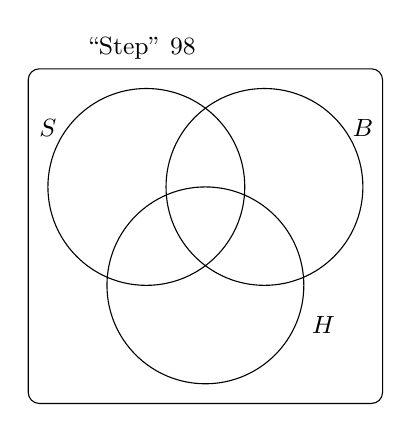
\begin{tikzpicture}[x=5mm, y=5mm,font=\small]

\draw[rounded corners] (0,-5.5) rectangle (9,3) (4.5,3)node[above, anchor=south east] {``Step'' 98};

\draw(3,0) circle (2.5);
\draw(6,0) circle (2.5);
\draw(4.5,-2.5) circle (2.5);

\node at (.5,1.5) {$S$};
\node at (8.5,1.5) {$B$};
\node at (7.5,-3.5) {$H$};

\end{tikzpicture}

\end{center}
$S$ è l'insieme degli iscritti al corso di Salsa, $B$ l'insieme degli iscritti 
al corso di
Break Dance, $H$ l'insieme degli iscritti al corso di Hip Hop.
\end{esercizio}

\begin{esercizio}
\label{ese:7.26}
Il club ``Argento vivo'' ha~2500 iscritti; nel mese di gennaio ha organizzato 
alcune
manifestazioni sportive alle quali hanno partecipato~850 degli iscritti
e alcuni tornei di scacchi ai quali hanno partecipato in~780. 320
iscritti al club hanno potuto partecipare, grazie alla perfetta
organizzazione, sia alle manifestazioni sportive sia ai tornei di
scacchi. Quanti soci del club non hanno partecipato a nessuna delle
iniziative e quanti invece hanno partecipato ad almeno una?
\end{esercizio}

\begin{esercizio}[\Ast]
 \label{ese:7.27}
In una scuola di musica si tengono~4 corsi di cui quello di pianoforte è 
obbligatorio
per tutti i~100 studenti iscritti, mentre quelli di violino, flauto e
chitarra sono facoltativi. Per essere ammessi agli esami di fine anno
bisogna frequentare almeno un corso oltre a quello di pianoforte. Se gli alunni:

\begin{enumeratea}
 \item che frequentano il corso di flauto sono~25 e non frequentano né quello di 
violino, né quello di chitarra;
 \item iscritti sia al corso di violino sia a quello di chitarra sono~20;
 \item che frequentano il corso di violino sono~46;
 \item che frequentano solo il corso di violino sono tanti quanti quelli che 
frequentano solo il corso di chitarra.
\end{enumeratea}

Quanti alunni non possono sostenere l'esame finale?
Quale dei seguenti diagrammi di Venn può essere preso come modello della 
situazione?
\begin{center}
 % (c) 2012 Dimitrios Vrettos - d.vrettos@gmail.com
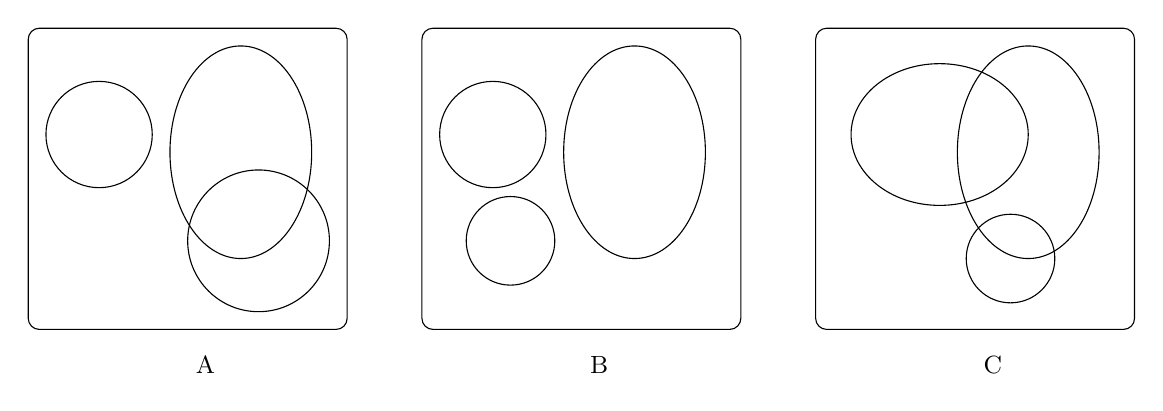
\begin{tikzpicture}[x=4.5mm, y=4.5mm,font=\small]

\draw[rounded corners] (0,-5.5) rectangle (9,3) (5,-6)node[below] {A};
\draw(2,0) circle (1.5);
\draw (6,-.5)ellipse (2 and 3);
\draw(6.5,-3) circle (2);

\begin{scope}[xshift=50mm]
\draw[rounded corners] (0,-5.5) rectangle (9,3) (5,-6)node[below] {B};
\draw(2,0) circle (1.5);
\draw (6,-.5)ellipse (2 and 3);
\draw(2.5,-3) circle (1.25);
\end{scope}

\begin{scope}[xshift=100mm]
\draw[rounded corners] (0,-5.5) rectangle (9,3) (5,-6)node[below] {C};
\draw(3.5,0) ellipse (2.5 and 2);
\draw (6,-.5)ellipse (2 and 3);
\draw(5.5,-3.5) circle (1.25);
\end{scope}
\end{tikzpicture}

\end{center}
\hfill [3; A]
\end{esercizio}

\begin{multicols}{2}
% \begin{esercizio}[\Ast]
% \label{ese:7.28}
% I componenti di una compagnia teatrale sanno almeno cantare, ballare,
% recitare. Al termine di una rappresentazione si sa che~12 hanno almeno
% ballato, 8 hanno almeno cantato e~16 hanno almeno recitato. La
% versatilità dei componenti ha permesso che~5 abbiano almeno ballato e
% cantato, 3 abbiano almeno cantato e recitato, 8 abbiano ballato e
% recitato, 2 ballerini hanno ballato, cantato e recitato. Quanti sono i
% componenti della compagnia?
% \end{esercizio}
% \hfill [22]
% 
% \begin{esercizio}[\Ast]
% \label{ese:7.29}
% Da un'indagine condotta su consumatori adulti è
% risultato che~605 bevono almeno vino, 582 bevono almeno latte, 348
% bevono almeno birra, 140 bevono almeno vino e birra, 85 bevono almeno
% vino e latte, 56 bevono almeno latte e birra, 25 bevono tutte e tre le
% bevande mentre~71 non bevono alcuna delle bevande citate.
% \begin{enumeratea}
% \item Quante persone bevono una sola bevanda?
% \item quante bevono almeno una bevanda?
% \item quante sono le persone intervistate?
% \end{enumeratea}
% \end{esercizio}
% \hfill [a)~1048,\quad b)~1279,\quad c)~1350]
% 
% \begin{esercizio}[\Ast]
% \label{ese:7.30}
% In una scuola di lingue sono iscritti~164 studenti; 80 seguono il
% corso di francese e~120 il corso di tedesco. Quanti studenti seguono
% entrambi i corsi? Quanti studenti seguono
% solo il corso di tedesco?
% \end{esercizio}
% \hfill [36; 84]

\begin{esercizio}
\label{ese:7.31}
In un classe di~28 allievi, 18 frequentano il laboratorio di teatro,
22 il laboratorio di fotografia, 3 non frequentano alcun laboratorio.
Rappresenta la situazione con un diagramma di Eulero-Venn. Quanto
allievi frequentano entrambi i laboratori? Quanti frequentano almeno un
laboratorio? Quanti non frequentano il laboratorio di teatro?
\end{esercizio}

\begin{esercizio}
\label{ese:7.32}
In una pizzeria, domenica sera, erano presenti~140 persone: 50 hanno
mangiato pizza e calzone, 20 hanno mangiato solo calzone e~15 non hanno
mangiato né pizza né calzone. Il pizzaiolo si chiede se può
conoscere in base alle precedenti informazioni, quante pizze ha
preparato. Aiutalo a risolvere il suo problema illustrando la
situazione con un diagramma di Venn, assegnando a ciascun insieme la
sua cardinalità.
\end{esercizio}

\begin{esercizio}
\label{ese:7.33}
In un paese di~3200 abitanti arrivano due quotidiani: il primo è letto da~850
persone, il secondo da~780. Poiché~320 persone leggono entrambi i
quotidiani, quante persone non leggono alcun quotidiano e quante almeno uno?
\end{esercizio}

\begin{esercizio}[Test di ammissione a architettura~2008]
\label{ese:7.34}
Nella classe di Asdrubale ci sono~37 allievi. Tutti si sono iscritti
ad almeno una delle due attività extracurriculari (musica e
pallavolo). Alla fine~15 fanno musica e~28 fanno pallavolo.
Quanti allievi, frequentando entrambe le attività, hanno la
necessità di programmare gli orari per evitare sovrapposizioni?
\begin{center}
 \boxA~13\quad\boxB~9\quad\boxC~16\quad\boxD~22\quad\boxE~6
\end{center}
\end{esercizio}

\begin{esercizio}[Test di ammissione a medicina~2008]
\label{ese:7.35}
In un'aula scolastica, durante la ricreazione, 14
studenti stanno seduti, 8 mangiano la pizza. Con questi dati si può
concludere con certezza che il numero totale~$N$ degli studenti è:
\begin{center}
 \boxA\quad~$N>14$\quad\boxB\quad~$N<14$\quad\boxC\quad~$N>22$\quad\boxD\quad~$N 
= 22$\quad\boxE\quad~$N\geqslant~14$
\end{center}
\end{esercizio}

\begin{esercizio}
\label{ese:7.36}
In una scuola di~150 alunni ci sono~23 studenti che frequentano il corso ECDL, 
41 studenti che frequentano solo il corso di Inglese, 3
studenti che frequentano tutti e due i corsi. Quanti sono gli studenti che 
frequentano solo il corso ECDL? Quanti studenti non frequentano
nessuno dei due corsi?
\end{esercizio}

\begin{esercizio}
\label{ese:7.37}
In un giorno di vacanza, 20 alunni dovrebbero studiare latino e
matematica per recuperare le lacune: 8 non studiano latino, 10 studiano
matematica e~4 non studiano niente. Quanti alunni studiano entrambe le
materie?
\end{esercizio}

\begin{esercizio}
\label{ese:7.38}
In una classe di~20 alunni si sta organizzando una gita
scolastica. Durante l'assemblea gli alunni raccolgono
informazioni sulle mete già visitate: 18 hanno visitato Venezia, 14
Roma, 5 Firenze. Solo~3 hanno visitato tutte e tre le città, 5 hanno
visitato Firenze e Venezia, 3 solo Venezia. Quanti hanno visitato solo
Firenze? Quanti hanno visitato Firenze e Roma? Quanti non hanno
visitato nessuna delle tre città? Quanti non hanno visitato Roma?
\end{esercizio}
\end{multicols}

\subsection{Esercizi riepilogativi}

\begin{esercizio}
\label{ese:6.23}
Scrivi i primi dieci elementi dei seguenti insiemi.
\begin{multicols}{2}
\begin{enumeratea}
\spazielenx
\item $A=\{x/x=2n, n\in\insN\}$
\item $B=\{x/x=n^{2}, n\in\insN\}$
\item $C=\{x/x=2n^{2}, n\in\insN\}$
\item $D=\{x/x=2n+2, n\in\insN\}$
\item $E=\{x/x=n^{2}-n, n\in\insN\}$
\item $E=\{x/x=\dfrac{n+1}{n-1}, x\in\insZ, n\in\insN \}$
\end{enumeratea}
\end{multicols}
\end{esercizio}

\begin{esercizio}
\label{ese:6.24}
Rappresenta i seguenti insiemi con rappresentazione tabulare, caratteristica e 
grafica.
\begin{enumeratea}
\item Insieme~$A$ dei divisori di~30;
\item insieme~$B$ dei numeri pari minori o uguali a~10;
\item l'insieme~$C$ delle province della Puglia;
\item l'insieme~$D$ delle lettere della parola ``COCCO''.
\end{enumeratea}
\end{esercizio}

\begin{esercizio}
\label{ese:6.25}
Rappresenta nel modo che ritieni più opportuno gli insiemi i cui elementi sono:
\begin{enumeratea}
\item i numeri naturali multipli di~5 compresi tra~10 e~10000;
\item i colori dell'arcobaleno;
\item i numeri razionali maggiori o uguali a~2/7;
\item i punti di una superficie~$S$
\item le lettere di cui è composto il tuo nome.
\end{enumeratea}
\end{esercizio}

\begin{esercizio}
\label{ese:6.26}
Rappresenta con una modalità a tua scelta l'insieme dei numeri interi multipli 
di~5 maggiori di~10 e minori di~100 che non
sono dispari.
\end{esercizio}

\begin{esercizio}
\label{ese:6.27}
Dati gli insiemi:~$X=\{8, 9, 10\}$, $Y=\{0, 8, 9, 10\}$, $H=\{10, 9, 8\}$,
$W=\{w\in\insN/\ 8\le w\le~10\}$, $Z=\{z\in\insN/\ 8<z\le10\}$ 
e~$J=\{j\in\insN/\ 7<j<11\}$,
individua le uguaglianze corrette.
\begin{multicols}{3}
\begin{enumeratea}
\item $X = Y$
\item $X= H$
\item $W = H$
\item $X = Z$
\item $\card Z=2$
\item $X = J$
\end{enumeratea}
\end{multicols}
\end{esercizio}

\begin{esercizio}
\label{ese:6.28}
Dati gli insiemi:
$A=$\{g, a, t, o\}, $B=$\{o, g, t, a\}, $C=\{c/c$ è una lettera della parola 
``gatto''\},
$D=$\{g, t\}, $E=$\{gatto\}, $F=\{f / f$ è una consonante della parola 
``gatto''\},
segna con una crocetta le uguaglianze corrette:
\begin{multicols}{4}
\begin{enumeratea}
 \item $A = B$
 \item $A = D$
 \item $A = C$
 \item $E = A$
 \item $C = E$
 \item $D = F$
 \item $C = D$:
 \item $D = E$
 \columnbreak
 \item $\card C=5$
 \item $\card E=5$
\end{enumeratea}
\end{multicols}
\end{esercizio}

\begin{esercizio}
\label{ese:6.29}
Per ciascuno dei seguenti insiemi indica alcuni elementi.
\TabPositions{6cm}
\begin{enumeratea}
\item $X=\{x\in\insN/\ x-1\text{ è pari }\}$\dotfill
\item $Y=\{y\in\insN/\ y=3n,\text{ con }\ n\in\insN\}$\dotfill
\item $Z=\{z\in\insN/\ z=3n\text{ e } z\text{ non è divisibile per 
}\;2,n\in\insN\}$\dotfill
\item $W=\{w\in\insN/\ w<0\}$\dotfill
\end{enumeratea}
\end{esercizio}

\begin{esercizio}
\label{ese:6.30}
Quali delle seguenti scritture sono vere?
\begin{multicols}{2}
\begin{enumeratea}
% \TabPositions{7cm}
\item $5\in \{10,8,6,4,2\}$\hfill\boxV\quad\boxF
\item $15\in \{n\in\insN/n\geqslant~10\}$\hfill\boxV\quad\boxF
\item $7\in \{n\in\insN/n+5<10\}$\hfill\boxV\quad\boxF
\item $l\notin\{x/x\text{ appartiene a ``scuola''}\}$\hfill\boxV\quad\boxF
\end{enumeratea}
\end{multicols}
\end{esercizio}

\begin{esercizio}
\label{ese:6.31}
Quali dei seguenti insiemi sono uguali?
\begin{multicols}{2}
 \begin{enumeratea}
 \item $A=\{1+3, 5-2, 1+1, 9-8, 1-1\}$
\item $B=\{n\in\insN/n<5\}$
\item $C=\{6-4, 6+4, 6-6\}$
 \end{enumeratea}
\end{multicols}
\end{esercizio}

% \newpage

\begin{esercizio}
\label{ese:6.32}
Quali dei seguenti insiemi sono uguali?
\begin{multicols}{2}
\begin{enumeratea}
\item $A=\{x\in\insN/\ 3\leqslant x\leqslant~12\}$
\item $B=\{x\in\insN/x=3n\ \text{ con } 1\leqslant n\leqslant~4\}$
\item $A=\{x\in\insN/\ 2<x<13\}$
\item $B=\{x\in\insN/x=3^{n}\text{ con }n=1,2,3,4\}$
\end{enumeratea}
\end{multicols}
\end{esercizio}

\begin{esercizio}
\label{ese:7.39}
Siano~$A=\{x\in\insN/1\leqslant x\leqslant~15\}$ e~$B=\{x\in\insN/2\leqslant 
x\leqslant~20\}$
\begin{center}
% (c) 2012 Dimitrios Vrettos - d.vrettos@gmail.com
\begin{tikzpicture}[x=3mm, y=5mm,font=\small]

\draw[->, thick] (-1,0)--(24,0) node [above left] {$\insN$};
\draw[pattern =north east lines, pattern color=RedOrange] (1,0) rectangle (15,1) (1,1)node[left] {$A$};
\draw[pattern =north west lines, pattern color=CornflowerBlue] (2,0) rectangle (20,1.5) node[right]{$B$};

\foreach \x/\xtext in {1/1,2/2,15/15,20/20}
\draw[fill] (\x,0)circle (1pt) (\x,0)node [below]{\xtext};
\end{tikzpicture}

\end{center}
Quale delle seguenti affermazioni è vera:
\begin{center}
\boxA\quad~$A\subset B$\quad\boxB\quad~$B\supset 
A$\quad\boxC\quad$A=B$\quad\boxD\quad$B\not\subset A$
\end{center}
\end{esercizio}

\begin{esercizio}
\label{ese:7.40}
 Siano~$A=\{x\in\insN/x \text{ è pari e }(1\leqslant x\leqslant~20)\}$ 
e~$B=\{x\in\insN/x \text{ è multiplo di~6 e }(2\leqslant x\leqslant~18)\}$
Quale affermazione è vera?
\begin{center}
 \boxA\quad~$A\subset B$\quad\boxB\quad~$B\supset 
A$\quad\boxC\quad~$A=B$\quad\boxD\quad~$B\subset A$
\end{center}
\end{esercizio}

\begin{esercizio}
\label{ese:7.41}
Siano~$A=\{x\in\insN/3\leqslant x\leqslant~10\}$ e~$B=\{x\in\insN/2\leqslant 
x\leqslant~20\}$
Quali delle seguenti affermazioni è vera:
\begin{center}
 \boxA\quad~$A\subset B$\quad\boxB\quad~$B\supset 
A$\quad\boxC\quad~$A=B$\quad\boxD\quad~$B\not\subset A$
\end{center}
\end{esercizio}

\begin{esercizio}
\label{ese:7.42}
Individua tutti i possibili sottoinsiemi propri formati da tre elementi 
dell'insieme~$C=$\{a, e, i, o, u\}.
\end{esercizio}

\begin{esercizio}
\label{ese:7.43}
Sia~$A=\{1,2,3,4\}$ scrivi i possibili sottoinsiemi propri e impropri di~$A$
\end{esercizio}

\begin{esercizio}
\label{ese:7.44}
Associa a ogni diagramma la corretta rappresentazione grafica. Attenzione ci può 
essere più di una risposta corretta.
\begin{multicols}{2}
% \TabPositions{5cm}
\begin{enumeratea}
 \item $M\subset P$ \hfill\boxA\quad\boxB\quad\boxC\quad\boxD\quad\boxE
\item $P\supseteq M$ \hfill\boxA\quad\boxB\quad\boxC\quad\boxD\quad\boxE
\item $M\subseteq (M\cup P)$ \hfill\boxA\quad\boxB\quad\boxC\quad\boxD\quad\boxE
\item $M\not\subset P$ \hfill\boxA\quad\boxB\quad\boxC\quad\boxD\quad\boxE
\item $P\subset (P\cup M)$ \hfill\boxA\quad\boxB\quad\boxC\quad\boxD\quad\boxE
\item $M\neq P$ \hfill\boxA\quad\boxB\quad\boxC\quad\boxD\quad\boxE
\end{enumeratea}
\end{multicols}
\begin{center}
% (c) 2012 Dimitrios Vrettos - d.vrettos@gmail.com
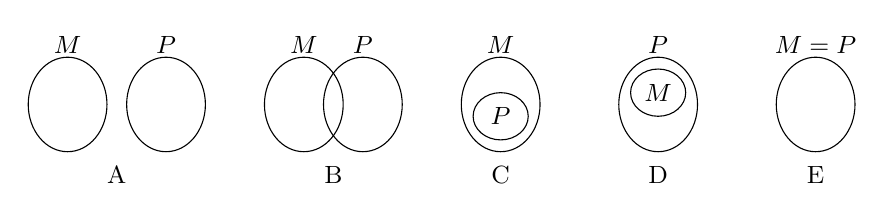
\begin{tikzpicture}[x=5mm, y=3mm,font=\small]

\draw (0,0) ellipse (1 and 2) (0,2.5)node {$M$};
\draw (2.5,0) ellipse (1 and 2)(2.5,2.5) node {$P$};
\node  at (1.25,-3) {A};

\begin{scope}[xshift=30mm]
\draw (0,0) ellipse (1 and 2) (0,2.5)node {$M$};
\draw (1.5,0) ellipse (1 and 2)(1.5,2.5) node {$P$};
\node  at (.75,-3) {B};
\end{scope}

\begin{scope}[xshift=55mm]
\draw (0,0) ellipse (1 and 2) (0,2.5)node {$M$};
\draw (0,-.5) ellipse (.7 and 1) node {$P$};
\node  at (0,-3) {C};
\end{scope}

\begin{scope}[xshift=75mm]
\draw (0,0) ellipse (1 and 2) (0,2.5)node {$P$};
\draw (0,.5) ellipse (.7 and 1) node {$M$};
\node  at (0,-3) {D};
\end{scope}

\begin{scope}[xshift=95mm]
\draw (0,0) ellipse (1 and 2) (0,2.5)node {$M=P$};
\node  at (0,-3) {E};
\end{scope}
\end{tikzpicture}

\end{center}
\end{esercizio}
% \newpage

\begin{esercizio}
\label{ese:7.45}
Determina l'unione tra i seguenti insiemi.

\begin{enumeratea}
 \item $A=\{-3,-2,-1,0,+1,+2,+3\}$, $B=\{-2,-1,0,+1,+2,+3,+4\}$ $A\cup 
B=\dotfill$
 \item $A=\{x\in\insN/2\le x\le~5\}$, $B=\{x\in\insN/3<x<7\}$ $A\cup B=\dotfill$
 \item $A=\{x\in\insZ/-5\le x\le +5\}$, $B=\{x\in\insZ/-15\le x<3\}$ $A\cup 
B=\dotfill$
 \item $A=\{x\in\insN/x>100\}$, $B=\{x\in \insN/10<x<20\}$ $A\cup B=\dotfill$
 \item $A=\{l\text{ lettera di SATURNO}\}$, $B=\{l\text{ lettera di NETTUNO}\}. 
A\cup B=\dotfill$
\end{enumeratea}
\end{esercizio}

\begin{esercizio}
\label{ese:7.46}
Sia~$M_{3}$ l'insieme dei multipli~3 e~$M_{4}$ l'insieme dei multipli di~4, in
generale~$M_{n}$ l'insieme dei multipli del numero~$n$

 \begin{enumeratea}
 \item Calcola~$M_{3}\cap M_{4}$ Si tratta di~$M\ldots$ l'insieme dei multipli 
di \ldots;
 \item calcola~$M_{6}\cap M_{4}$ Si tratta di~$M\ldots$ l'insieme dei multipli 
di \ldots;
 \item calcola~$M_{60}\cap M_{48}$
 \item sai dedurre una regola che, dati due numeri naturali~$m$ e~$n$ 
calcoli~$M_{m}\cap M_{n}$? Può accadere che questo insieme sia vuoto?
 \end{enumeratea}
\end{esercizio}


\begin{esercizio}
\label{ese:7.47}
Sia~$D_{4}$ l'insieme dei divisori di~4 e~$D_{6}$ l'insieme dei divisori di~6, 
in
generale~$D_{n}$ l'insieme dei divisori del numero~$n$

\begin{enumeratea}
 \item Calcola~$D_{4}\cap D_{6}$ Si tratta di~$D\ldots$ l'insieme dei divisori 
di \ldots;
 \item calcola~$D_{60}\cap D_{48}$
 \item sai dedurre una regola che, dati due numeri naturali~$m$ e~$n$,
calcoli~$D_{m}\cap D_{n}$? Può accadere che questo insieme sia
vuoto? Qual è il numero minimo di elementi che può contenere?
\end{enumeratea}
\end{esercizio}

\begin{esercizio}
\label{ese:7.48}
$A=\{x/x\in \insQ,0<x<\dfrac{3}{2}\}$ e~$B=\{x/x\in \insQ,1<x<6\}$, 
calcola~$A\cap B=\ldots$
\end{esercizio}

\begin{esercizio}
\label{ese:7.49}
$A=\{x/x\in \insQ,-1<x<0\}$ e~$B=\{x/x\in \insQ,\dfrac{1}{3}<x<6\}$, 
calcola~$A\cap B=\ldots$
\end{esercizio}

\begin{esercizio}
\label{ese:7.50}
$A=\{x/x\in \insQ,-5<x<10\}$ e~$B=\{x/x\in \insQ,\dfrac{1}{3}<x<6\}$, 
calcola~$A\cap B=\ldots$
\end{esercizio}

\begin{esercizio}
\label{ese:7.51}
$A=\{x/x\in \insQ,0\le x<10\}$ e~$B=\{x/x\in \insQ,\dfrac{1}{3}<x\le~6\}$, 
calcola~$A\cap B=\ldots$
\end{esercizio}

\begin{esercizio}
\label{ese:7.52}
Dato l'insieme~$A=\{3, 4, 5, 6, 7, 8, 9, 12, 32\}$ e il suo sottoinsieme~$B$ dei 
multipli di~3, determina gli
insiemi~$A-B$ e~$B-A$
\end{esercizio}

\begin{esercizio}
\label{ese:7.53}
Dato l'insieme~$X=\{x\in N/10\le x\le~100\}$ e~$Y=\{y\in N/10<y<100\}$ 
determina~$X-Y$ e~$Y-X$
\end{esercizio}

\begin{esercizio}
\label{ese:7.54}
Determina la differenza tra i seguenti insiemi:

\begin{enumeratea}
 \item $A=\{-3,-2,-1,0,+1,+2,+3\}$, $B=\{-2,-1,0,+1,+2,+3,+4\}$ $A-B=\ldots$
\item $A=\{x\in\insN/2\le x\le~5\}$, $B=\{x\in\insN/3<x<7\}$ $B-A=\ldots$
\item $A=\{x\in\insZ/-5\le x\le +5\}$, $B=\{x\in\insZ/-15\le x<3\}$ $A-B=\ldots$
\item $A=\{x\in\insN/x>100\}$, $B=\{x\in \insN/10<x<20\}$ $B-A=\ldots$
\item $A=\{l\text{ lettera di SATURNO}\}$, $B=\{l\text{ lettera di NETTUNO}\}$ 
$A-B=\ldots$
\end{enumeratea}
\end{esercizio}

\begin{esercizio}
\label{ese:7.55}
Dati gli insiemi~$C$ e~$D$ tali che~$C\subset D$
completa le seguenti relazioni aiutandoti con la rappresentazione
grafica
\begin{multicols}{3}
\begin{enumeratea}
\item $D-C=$
\item $D\cap \overline{C}=$
\item $\overline{{C\cap D}}=$
\item $C\cup \overline{C}=$
\item $C-D=$
\item $C\cap \overline{C}=$
\end{enumeratea}
\end{multicols}
\end{esercizio}

\begin{esercizio}
\label{ese:7.56}
Quale delle seguenti scritture corrisponde a~$\overline{{X\cap \overline{Y}}}$:
\begin{multicols}{4}
 \begin{enumeratea}
 \item $\overline{X}\cup \overline{Y}$
 \item $\overline{X}\cap \overline{Y}$
 \item $\overline{X}\cup Y$
 \item $X\cup \overline{Y}$
 \end{enumeratea}
\end{multicols}
\end{esercizio}


\begin{esercizio}
\label{ese:7.57}
Esegui le operazioni indicate~$A\cup B$, $A\cap B$, $A-B$

\begin{enumeratea}
\item $A=\{2,4,6,8\}$ $B=\{1,3,6,9\}$
\item $A=$\{a,e,i,o,u\} $B=$\{a,b,c,d,e\}
\item $A=\emptyset $ $B=\{0\}$
\item $A=\{x\in\insN/ x\text{ è pari}\}$ $B=\{x\in\insN/ x\text{ è dispari}\}$
\item $A=\{x\in\insN/ x\text{ è multiplo di~2}\}$ $B=\{x\in\insN/ x\text{ è 
multiplo di~4}\}$
\item $A=\{x\in\insZ/-5\le x\le~5\}$ $B=\{x\in\insZ/-2\le x\le~8\}$
\item $A=\{x\in\insN/ x\text{ è lettera di casa}\}$ $B=\{x\in\insN/ x\text{ è 
lettera di caserma}\}$
\end{enumeratea}
\end{esercizio}

\begin{multicols}{2}
 
\begin{esercizio}
\label{ese:7.58}
Dato~$A=\{x\in\insN/ x\text{ è multiplo di~2}\}$ 
determina~$\complement_{\insN}A$
\end{esercizio}


\begin{esercizio}
\label{ese:7.59}
Dato~$A=\{I, II, III\}$ e~$B=\{a,b\}$ determina~$A\times B$
\end{esercizio}

\begin{esercizio}
\label{ese:7.60}
Dato~$B=\{1,2,3\}$ calcola~$(B\cup B)\cap B$
\end{esercizio}

\begin{esercizio}
\label{ese:7.61}
$A=$\{2, 4, 6, 8, 10, 12, 14, 16, 18, 20\}, $B=$\{3, 6, 9, 12, 15, 18\},
$C=$\{1, 3, 5, 7, 9, 11, 13, 15, 17, 19\} calcola
$A\cap B$, $A\cup C$, $(A\cap B)\cup C$, $B\cap C$, $(A\cup B)\cap(B\cup C)$
\end{esercizio}

\begin{esercizio}
\label{ese:7.62}
$A=\{x\in\insZ/-5\le x<2\}$, $B=\{x\in\insN/-3<x\le~2\}$ calcola
$A\cup B$, $A\cap B$, $B-A$, $\complement_{A}B$, $A\times(A\cap B)$ e~$\wp 
(B-A)$
\end{esercizio}

\begin{esercizio}
\label{ese:7.63}
Per ciascuna delle seguenti affermazioni false dai un controesempio.

\begin{enumeratea}
 \item $A\cup B=A$
\item $A\cap B=\emptyset \Rightarrow A=\emptyset $
\item se~$x$ è multiplo di~2 allora è anche multiplo di~4;
\item se~$\card A =2$ e~$\card B = 5$ allora~$\card A\cup B=7$
\item se~$\card A =2$ e~$\card B = 5$ allora~$\card A\cap B=2$
\end{enumeratea}
\end{esercizio}

\begin{esercizio}
\label{ese:7.64}
In base alla figura rispondi alle domande:
% \begin{multicols}{2}
\TabPositions{4.5cm}
\begin{enumeratea}
\item L'insieme~$E$ ha~5 elementi \tab\boxV\quad\boxF
\item $2\in E$ \tab\boxV\quad\boxF
\item $3\notin G$ \tab\boxV\quad\boxF
\item $F\subset G$ \tab\boxV\quad\boxF
\item $F\subset E$ \tab\boxV\quad\boxF
\item $\emptyset \subseteq G$ \tab\boxV\quad\boxF
\item $\card(E)=8$ \tab\boxV\quad\boxF
\item $10\in E$ \tab\boxV\quad\boxF
\item $F\cap E=F$ \tab\boxV\quad\boxF
\item $F\cup G=E$ \tab\boxV\quad\boxF
\item $(E-F)-G=\{1,4\}$ \tab\boxV\quad\boxF
\end{enumeratea}
\begin{center}
 % (c) 2012 Dimitrios Vrettos - d.vrettos@gmail.com
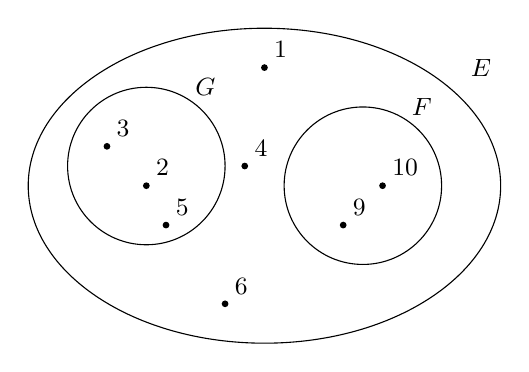
\begin{tikzpicture}[x=5mm, y=5mm,font=\small]

\draw (0,0) ellipse (6 and 4) (5.5,3)node {$E$};
\draw (2.5,0) circle (2)(4,2) node {$F$};
\draw (-3,.5) circle (2)(-1.5,2.5) node {$G$};

\draw[fill](-3,0) circle (1pt ) node[above right]  {2};
\draw[fill](-2.5,-1) circle (1pt ) node[above right]  {5};
\draw[fill](-4,1) circle (1pt ) node[above right]  {3};

\draw[fill](3,0) circle (1pt ) node[above right]  {10};
\draw[fill](2,-1) circle (1pt ) node[above right]  {9};

\draw[fill](0,3) circle (1pt ) node[above right]  {1};
\draw[fill](-.5,.5) circle (1pt ) node[above right]  {4};
\draw[fill](-1,-3) circle (1pt ) node[above right]  {6};
\end{tikzpicture}

\end{center}
% \end{multicols}
\end{esercizio}

\end{multicols}

% \begin{esercizio}
% \label{ese:7.65}
% Dato l'insieme~$A=\{0; 1; 5; 6; 9\}$ stabilisci
% quali dei seguenti sono o no suoi sottoinsiemi, completando con gli
% opportuni simboli le scritture a fianco indicate.
% \begin{multicols}{2}
% \TabPositions{3cm}
% \begin{enumeratea}
% \item $B=\{1; 5; 6\}$ \tab $B\ldots\ldots\ldots A$
% \item $C=\{0; 1; 3; 5\}$ \tab $C \ldots\ldots\ldots A$
% \item $D=\{ \}$ \tab $D \ldots\ldots\ldots A$
% \item $E=\{0\}$ \tab $E \ldots\ldots\ldots A$
% \item $F=\{5; 6; 7\}$ \tab $F \ldots\ldots\ldots A$
% \item $G=\{6; 0; 1; 5; 9\}$ \tab $G\ldots\ldots\ldots A$
% \end{enumeratea}
% \end{multicols}
% \end{esercizio}
% 
% \begin{esercizio}
% \label{ese:7.66}
% Siano dati i seguenti insiemi~$C=\{x/x$ è una lettera della parola ``REMARE''\}, 
% $D=\{x/x$ è una lettera della parola ``VOLARE''\},
% $E=\{x/x$ è una lettera della parola ``AMARE''\},
% indica quali delle seguenti relazioni sono vere:
% \begin{center}
% \boxA\quad~$D\subseteq C$\quad\boxB\quad~$D\not\subset 
% E$\quad\boxC\quad~$C=E$\quad\boxD\quad~$E\supseteq C$
% \end{center}
% \end{esercizio}

\begin{esercizio}
\label{ese:7.67}
Completa la seguente tabella:

\begin{tabular*}{.9\textwidth}{@{\extracolsep{\fill}}*{2}{cl}}
\toprule
Simbologia & Significato\\
\midrule
$A=\{a,b,c,d\}$ & $A$ è formato dagli \dotfill~$a, b, c, d$\\
$a\in A$ & L'elemento~$a$ \dotfill all'insieme~$A$\\
\dotfill & L'elemento f non appartiene all'insieme~$A$\\
$B\subset A$ & L'insieme~$B$ è \ldots\ldots nell'insieme~$A$, ovvero~$B$ è un 
\ldots\ldots di~$A$\\
\dotfill & L'insieme vuoto è un sottoinsieme di~$A$\\
\dotfill & L'insieme~$C$ è l'unione degli insiemi~$A$ e~$B$\\
$D=A\cap B$ & L'insieme~$D$ è \dotfill degli insiemi~$A$ e~$B$\\
$A\cap F=\emptyset $& $A$ e~$F$ sono insiemi \dotfill cioè non hanno \dotfill \\
$L=\complement_{A}B$ & L'insieme~$L$ è \dotfill \\
\dotfill & L'insieme~$M$ è la differenza tra~$A$ e~$B$\\
\bottomrule
\end{tabular*}
\end{esercizio}

\begin{esercizio}
\label{ese:7.68}
Rappresenta graficamente l'insieme~$A=\{x\in \insN/x\le~25 \text{ e } x\text{ è 
pari}\}$ e
$B=\{x\in N/x\le~27\text{ e } x\text{ è multiplo di~4}\}$ e stabilisci 
se~$A\supseteq B$
\end{esercizio}

\begin{esercizio}
\label{ese:7.69}
Verifica usando i diagrammi di Eulero-Venn che se~$A\subset B$ e~$B\subset C$ 
allora~$A\subset C$ Le relazioni valgono
anche se il simbolo~${\subset}$ viene sostituito con~${\subseteq}$?
\end{esercizio}

\begin{esercizio}
\label{ese:7.70}
Dato~$A=\{\text{do, re, mi}\}$ determina l'insieme delle parti~$\wp (A)$
\end{esercizio}

\begin{esercizio}
\label{ese:7.71}
Considerato gli insiemi~$X=\{a,c,d,t,o\}$ e 
$Y=\{x/x\text{ è una vocale della parola ``CAROTA''}\}$
stabilisci se le seguenti affermazioni sono vere o false.

\TabPositions{8cm}
\begin{multicols}{3}
\begin{enumeratea}
\item $Y \subset X$ \hfill \boxV\quad\boxF
\item $\{a,t\}\not\subset \wp (X)$ \hfill \boxV\quad\boxF
\item $\{a,t\}\in \wp (X)$ \hfill \boxV\quad\boxF
\item $0\in X$ \hfill \boxV\quad\boxF
\item $\emptyset \in \wp (X)$ \hfill \boxV\quad\boxF
\item $X\in \wp (X)$ \hfill \boxV\quad\boxF
\end{enumeratea}
\end{multicols}
\end{esercizio}

% \newpage

\begin{esercizio}
\label{ese:7.72}
Se~$U$ è l'insieme universo degli italiani, $D$ l'insieme delle donne italiane,
$L$ l'insieme degli italiani laureati, $S$ l'insieme degli italiani sposati, 
cosa rappresentano
i seguenti insiemi?
\begin{multicols}{3}
\begin{enumeratea}
\item $\overline{D}$
\item $L\cap D$
\item $\overline{{L\cup D\cup S}}$
\item $L-S$
\item $\overline{{L}}\cap S$
\item $\overline{{L\cap D\cap S}}$
\end{enumeratea}
\end{multicols}
\end{esercizio}

\begin{esercizio}
\label{ese:7.73}
Quanti elementi ha~$\wp (H)$ sapendo che~$H$ ha~7 elementi?
\begin{center}
 
\boxA\quad~49\quad\boxB\quad~64\quad\boxC\quad~128\quad\boxD\quad~7\quad
\boxE\quad~14
\end{center}
\end{esercizio}

\begin{esercizio}
\label{ese:7.74}
Scrivi l'insieme che ha per insieme delle parti:
$\{\emptyset,\{\text{Mauro}\},\{\text{Mario}\}\{\text{Mauro, Mario}\}\}$
\end{esercizio}

\begin{esercizio}
\label{ese:7.75}
Se~$A\cup B=B$ cosa puoi dire di~$A$ e~$B$?
\begin{center}
 \boxA\quad~$B\subseteq A$\quad\boxB\quad~$A\notin B$\quad
 \boxC\quad~$A\subseteq B$\quad\boxD\quad~$A\subset B$\quad
 \boxE\quad$A\cap B=\emptyset $
\end{center}
\end{esercizio}

\begin{esercizio}
\label{ese:7.76}
Dati gli insiemi~$A=\{10, 20, 30, 40, 50\}$, $B=\{20, 30, 50\}$,
determina un insieme~$C$ tale che:
\begin{multicols}{4}
\begin{enumeratea}
 \item $B\cup C=A$
 \item $A\cap C=B$
 \item $C\cup C=B$
 \item $C\cap C=A$
\end{enumeratea}
\end{multicols}
\end{esercizio}

\begin{esercizio}
\label{ese:7.77}
Dati gli insiemi~$A=\{x\in\insN/x\le~10\text{ e }x\text{ pari}\}$,
$B=\{x\in\insN/x\le~20\text{ e }x\text{ divisibile per }4\}$,
$C=\{1,2\}$ determina~$(A\cap B)xC$
\end{esercizio}

\begin{esercizio}
\label{ese:7.78}
Dimostra la proprietà distributiva dell'intersezione rispetto l'unione annerendo 
gli spazi opportuni.
\begin{center}
 % (c) 2012 Dimitrios Vrettos - d.vrettos@gmail.com
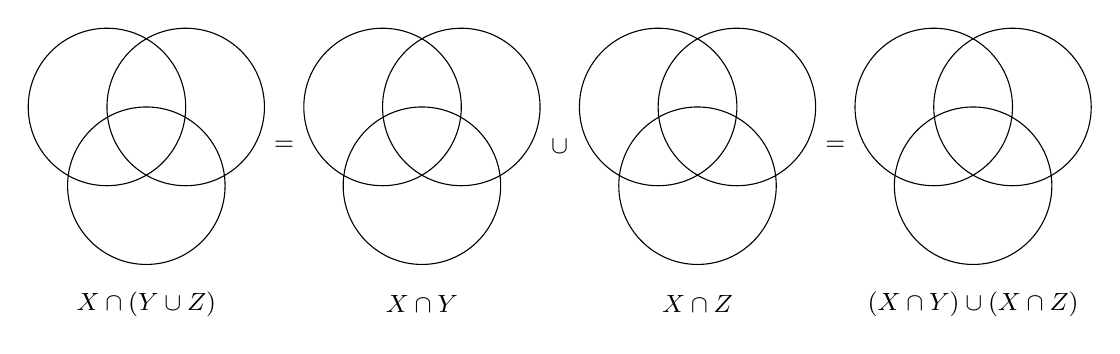
\begin{tikzpicture}[x=5mm, y=5mm,font=\small]

\draw (0,0) circle (2);
\draw (2,0) circle (2);
\draw (1,-2) circle (2);

\begin{scope}[xshift=35mm]
\draw (0,0) circle (2);
\draw (2,0) circle (2);
\draw (1,-2) circle (2);
\end{scope}

\begin{scope}[xshift=70mm]
\draw (0,0) circle (2);
\draw (2,0) circle (2);
\draw (1,-2) circle (2);
\end{scope}

\begin{scope}[xshift=105mm]
\draw (0,0) circle (2);
\draw (2,0) circle (2);
\draw (1,-2) circle (2);
\end{scope}

\foreach \x/\xtext in {4.5/=,11.5/\cup,18.5/=}
\node  at (\x,-1) {$\xtext$};

\foreach \xi/\xitext in {1/$X\cap(Y\cup Z)$,8/$X\cap Y$,15/$X\cap Z$,22/$(X\cap Y)\cup(X\cap Z)$}
\node  at (\xi,-5) {\xitext};
\end{tikzpicture}

\end{center}
\vspace{-12pt}
\end{esercizio}

\begin{esercizio}
\label{ese:7.79}
Se~$E-F=E$ cosa puoi dire di~$E$ e~$F$?
\begin{center}
 \boxA\quad~$E\cup F=E$\quad\boxB\quad~$E=F$\quad\boxC\quad~$E\subseteq 
F$\quad\boxD\quad~$F\subset E$\quad\boxE\quad~$E\cap F=\emptyset $
\end{center}
\end{esercizio}

\begin{esercizio}
\label{ese:7.80}
Dimostra la proprietà distributiva dell'unione rispetto l'intersezione annerendo 
gli spazi opportuni
e inserendo le formule opportune.
\begin{center}
 % (c) 2012 Dimitrios Vrettos - d.vrettos@gmail.com
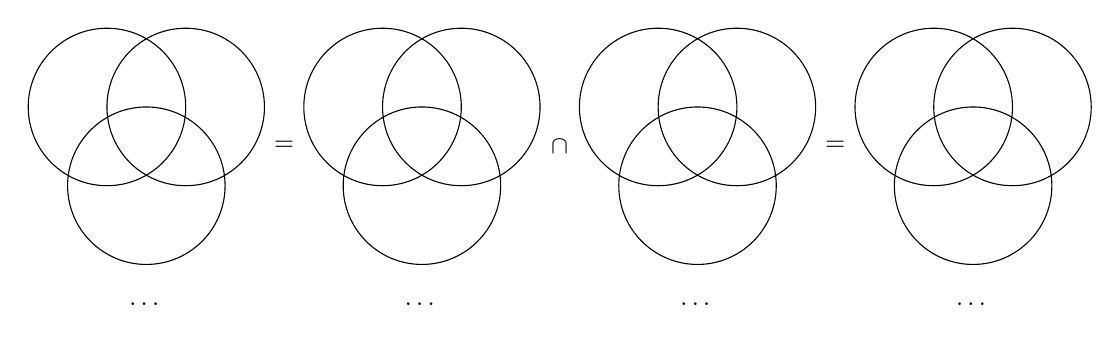
\begin{tikzpicture}[x=5mm, y=5mm,font=\small]

\draw (0,0) circle (2);
\draw (2,0) circle (2);
\draw (1,-2) circle (2);

\begin{scope}[xshift=35mm]
\draw (0,0) circle (2);
\draw (2,0) circle (2);
\draw (1,-2) circle (2);
\end{scope}

\begin{scope}[xshift=70mm]
\draw (0,0) circle (2);
\draw (2,0) circle (2);
\draw (1,-2) circle (2);
\end{scope}

\begin{scope}[xshift=105mm]
\draw (0,0) circle (2);
\draw (2,0) circle (2);
\draw (1,-2) circle (2);
\end{scope}

\foreach \x/\xtext in {4.5/=,11.5/\cap,18.5/=}
\node  at (\x,-1) {$\xtext$};

\foreach \xi in {1,8,15,22}
\node  at (\xi,-5) {\ldots};
\end{tikzpicture}

\end{center}
\vspace{-12pt}
\end{esercizio}

% \newpage

\begin{esercizio}
\label{ese:7.81}
Dati i seguenti insiemi~$A=\{x\in N/x\le~25\}$, $B=\{x\in N/4<x\le~9\}$, 
$C=\{x\in N/x<25\}$ e~$D=\{x\in N/x>7\}$. 
Scegli fra i seguenti i loro complementari.
\vspace{-6pt}
\begin{multicols}{2}
\begin{enumeratea}
\item $E=\{x\in N/x\ge~25\}$
\item $F=\{x\in N/x\le~6\}$
\item $G=\{x\in N/x>25\}$
\item $H=\{x\in N/x<7\}$
\item $I=\{x\in N/x<4\text{ e }x\ge~8\}$
\item $L=\{x\in N/x<4\text{ o }x\ge~10\}$
% \item $M=\{x\in N/x\le~4\text{ e }x\ge~9\}$
\end{enumeratea}
\end{multicols}
\vspace{-12pt}
\end{esercizio}

\begin{esercizio}
\label{ese:7.82}
Quali dei seguenti sono sottoinsiemi dei numeri pari? L'insieme dei
\vspace{-6pt}
\begin{center}
 \boxA\quad multipli di~4\quad\boxB\quad multipli di~3\quad\boxC\quad multipli 
di~6\quad\boxD\quad numeri primi
\end{center}
\vspace{-6pt}
\end{esercizio}

\begin{esercizio}
\label{ese:7.83}
In una classe di~32 allievi~14 hanno debito in matematica, 10 in
italiano, 16 non hanno avuto nessun debito. Rappresenta la situazione
con un diagramma di Eulero-Venn. Quanti allievi:
\vspace{-6pt}
\begin{multicols}{2}
\begin{enumeratea}
\item hanno debito in entrambe le materie;
\item hanno almeno un debito;
\item non hanno debito in italiano;
\item non hanno debito in matematica.
\end{enumeratea}
\end{multicols}
\vspace{-12pt}
% \hfill [a)~16,\quad b)~20,\quad c)~10,\quad d)~14]   ?????????????
\end{esercizio}

\begin{esercizio}
\label{ese:7.84}
Quali dei seguenti insiemi possono essere sottoinsiemi dell'insieme dei 
quadrilateri?
L'insieme dei:
\vspace*{-12pt}
\begin{multicols}{3}
\begin{enumeratea}
 \item quadrati;
 \item rombi;
 \item trapezi;
 \item triangoli equilateri;
 \item poligoni;
%  \item cerchi;
 \item parallelogrammi.
\end{enumeratea}
\end{multicols}
\vspace{-12pt}
\end{esercizio}

\begin{esercizio}
\label{ese:7.85}
Dati gli insiemi~$A=\{x/x\in\insN,x<10\}$, $B=\{x/x\in\insN,5<x\leqslant~16\}$,
$C=\{x/x\in \insN,x\geqslant~7\}$ determina:
\begin{multicols}{4}
\begin{enumeratea}
\item $A\cup B\cup C$
\item $A\cap B\cap C$
\item $(A\cup B)\cap C$
\item $(B\cap C)\cup A$
\end{enumeratea}
\end{multicols}
\end{esercizio}


\begin{esercizio}
\label{ese:7.86}
Dato~$A = \{x/x\text{ è un numero naturale, } x \text{ è pari e }x>12\}$ 
determina l'insieme complementare di~$A$
\end{esercizio}

\begin{esercizio}
\label{ese:7.87}
Quanti sono i sottoinsiemi dell'insieme che contiene come elemento
l'insieme vuoto?
\end{esercizio}

\begin{esercizio}
\label{ese:7.88}
$A=\{x/ x\text{ è divisore di }12\}$, $B=\{x / x\text{ è divisore di }6\}$,
$C=\{x / x\text{ è divisore di~15}\}$, determina:
\begin{multicols}{4}
 \begin{enumeratea}
 \item $A\cup B$
 \item $A\cup C$
 \item $A\cup B\cup C$
 \item $A\cap B$
 \item $B\cap C$
 \item $A\cap C$
 \item $A\cap B\cap C$
 \item $A\cap(B\cup C)$
 \end{enumeratea}
\end{multicols}
\end{esercizio}


\begin{esercizio}
\label{ese:7.89}
Dato l'insieme~$U=\{x/x=2n+1,n\in\insN,0\leqslant n\leqslant~5\}$:

\begin{enumeratea}
\item rappresenta~$U$ in forma tabulare;
\item costruisci due sottoinsiemi propri~$A$ e~$B$ di~$U$ tali che~$A\cap 
B=\emptyset $
\item determina~$A\cup B$ e~$A-B$, dai il risultato con rappresentazione 
tabulare e mediante diagrammi di
Eulero-Venn.
\end{enumeratea}
\end{esercizio}

% \newpage

\begin{esercizio}
\label{ese:7.90}
In base agli insiemi rappresentati con il diagramma di Eulero-Venn determina gli 
insiemi richiesti:
\begin{multicols}{2}
\begin{enumeratea}
\item $A\cup B$
\item $\overline{{A\cup B\cup C}}$
\item $A\cap B$
\item $B\cap C$
\item $A\cap B\cap C$
\item $A\cap (B\cup C)$
\item $A\cup (B\cap C)$
\item $B\cap \overline{C}$
\item $(A\cup B)-C$
\item $B\cap \overline{C}$
\item $C-(A\cap B)$
\item $\overline{{(A\cup B)}}-C$
\end{enumeratea}
\begin{center}
 % (c) 2012 Dimitrios Vrettos - d.vrettos@gmail.com
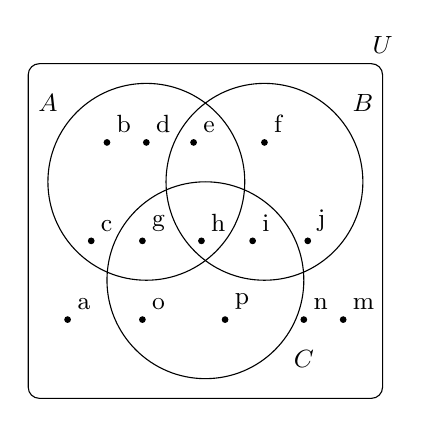
\begin{tikzpicture}[x=5mm, y=5mm,font=\small]

\draw[rounded corners] (-4,-5.5) rectangle (5,3) node[above] {$U$};
\draw (-1,0) circle (2.5) (-3.5,2)node {$A$};
\draw (2,0) circle (2.5) (4.5,2)node {$B$};
\draw (0.5,-2.5) circle (2.5) (3,-4.5)node {$C$};

\foreach \x/\xtext in {-2/b,-1/d,0.2/e,2/f}
\draw[fill] (\x,1)circle(1pt) node[above right]{\xtext};

\foreach \x/\xtext in {-2.4/c,-1.1/g,0.4/h,1.7/i, 3.1/j}
\draw[fill] (\x,-1.5)circle(1pt) node[above right]{\xtext};

\foreach \x/\xtext in {-3/a,-1.1/o,1/p,3/n, 4/m}
\draw[fill] (\x,-3.5)circle(1pt) node[above right]{\xtext};
\end{tikzpicture}

\end{center}
\end{multicols}
\end{esercizio}

\begin{multicols}{2}
\begin{esercizio}
\label{ese:7.91}
Determina l'insieme~$\wp(A)$, insieme delle parti di~$A$, dove $A$ è l'insieme 
delle lettere della parola ``NONNA''.
\end{esercizio}

\begin{esercizio}
\label{ese:7.92}
Nel seguente diagramma di Eulero-Venn gli insiemi~$r$, $s$, $t$
sono rette, gli elementi~$A$, $B$, $C$, $D$ sono punti. Dai una
rappresentazione geometria, rappresentando le rette e che corrispondono
alla seguente situazione.
\begin{center}
 % (c) 2012 Dimitrios Vrettos - d.vrettos@gmail.com
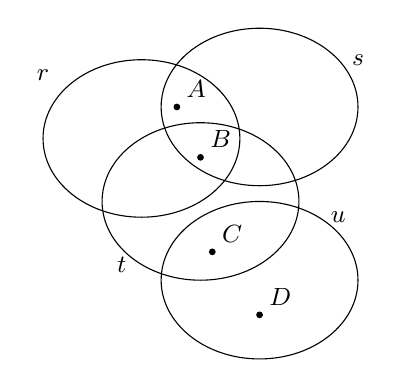
\begin{tikzpicture}[x=5mm, y=4mm,font=\small]
\draw (-1,0) circle (2.5) (-3.5,2)node {$r$};
\draw (2,1) circle (2.5) (4.5,2.5)node {$s$};
\draw (0.5,-2) circle (2.5) (-1.5,-4)node {$t$};
\draw (2,-4.5) circle (2.5) (4,-2.5)node {$u$};

\draw[fill] (-.1,1) circle (1pt) node[above right]  {$A$};
\draw[fill] (.5,-.6) circle (1pt) node[above right]  {$B$};
\draw[fill] (.8,-3.6) circle (1pt) node[above right]  {$C$};
\draw[fill] (2,-5.6) circle (1pt) node[above right]  {$D$};
\end{tikzpicture}

\end{center}
\end{esercizio}
\end{multicols}

